\documentclass{beamer}
\usepackage{comment}
\usepackage{physics}
\usetheme{Madrid}

\usepackage[utf8]{inputenc}
\usepackage{graphicx}

\title[Relativistic Dynamics]{Relativistic Behavior Detection through Electron Acceleration}
\author{Henry Shackleton}

\begin{document}

\titlepage

\section{Introduction and Theory}

\begin{frame}
  \frametitle{Classical Mechanics and Special Relativity Differ in Predictions}
  \textbf{Classical Mechanics}
  \begin{itemize}
    \pause
    \item Formalized by Newton in 1687
      \pause
    \item No limit to the speed of a particle
  \end{itemize}
\pause
  \textbf{Special Relativity}
  \begin{itemize}
    \pause
    \item Developed by Einstein in 1905
      \pause
    \item The speed of light, $c$, is constant in all reference frames
      \pause
    \item The velocity of any particle is capped at $c$
  \end{itemize}
\end{frame}

\begin{frame}
  \frametitle{Classical and Relativistic Kinetic Energies are Different}
  \textbf{Classical Kinetic Energy}
  \begin{equation*}
    K = \frac{p^2}{2m}
  \end{equation*}

  \pause
  \textbf{Relativistic Kinetic Energy}
  \begin{equation*}
    K = \sqrt{p^2 c^2 + m^2 c^4} - mc^2
  \end{equation*}
\end{frame}

\begin{frame}
  \frametitle{Electrons in Magnetic Fields are Accelerated in Circular Orbits}
  \begin{columns}
    \begin{column}{0.5\textwidth}
      \begin{itemize}
        \item
          $\dv{\vb{p}}{t} = e \left(\vb{E} + \frac{\vb{v}}{c} \times \vb{B}\right)$
        \item Electrons follow a circular orbit with radii proportional to their momentum
        \item $p = \frac{\rho e}{c} B$
      \end{itemize}
\end{column}
    \begin{column}{0.5\textwidth}
  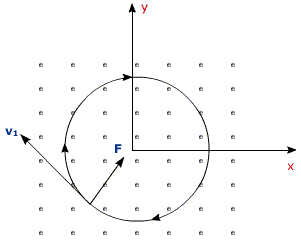
\includegraphics[width=6cm]{lorentz.png}
\end{column}
\end{columns}
\end{frame}

\begin{frame}
  \frametitle{Experimental Setup Constrains Radius of Electron Orbit}
  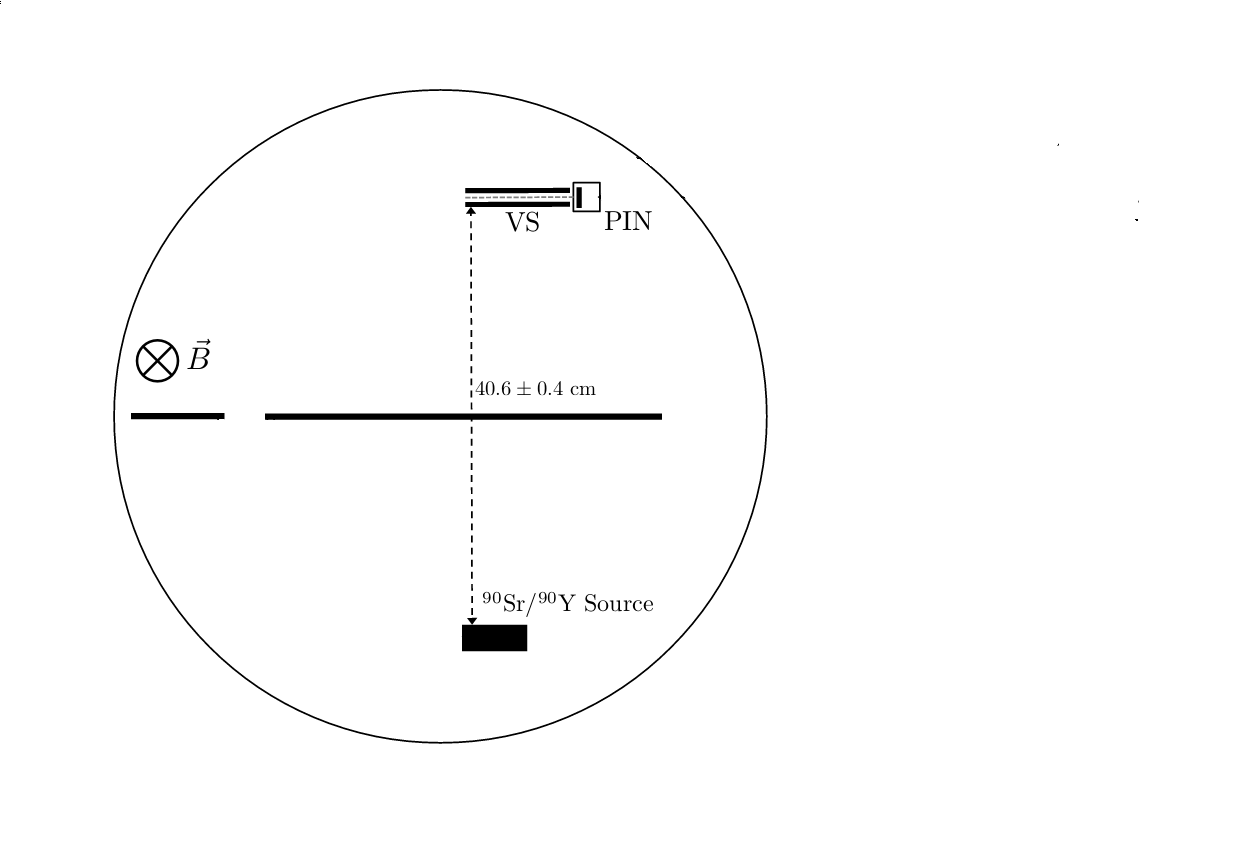
\includegraphics[width=11cm]{setup1.png}
\end{frame}

\begin{frame}
  \frametitle{Experimental Setup Constrains Radius of Electron Orbit}
  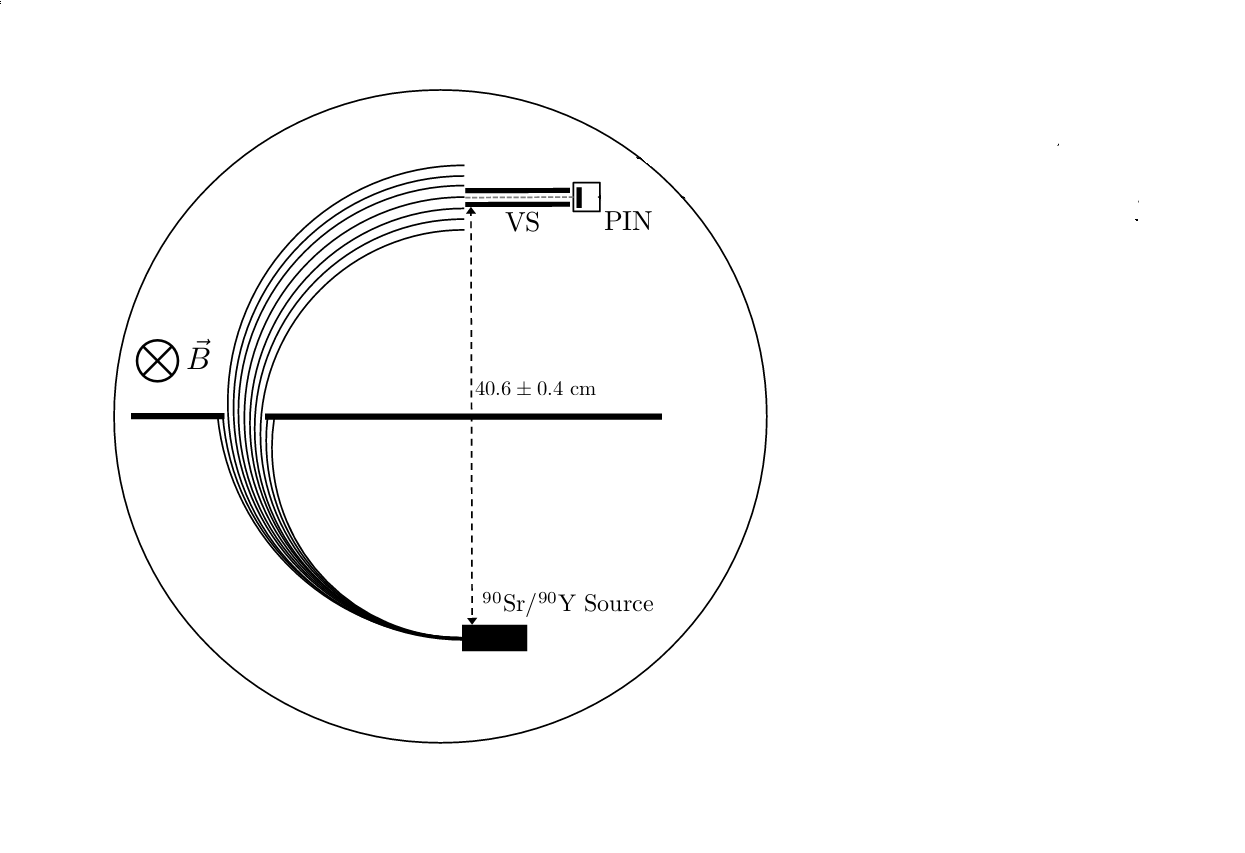
\includegraphics[width=11cm]{setup2.png}
\end{frame}

\begin{frame}
  \frametitle{Experimental Setup Constrains Radius of Electron Orbit}
  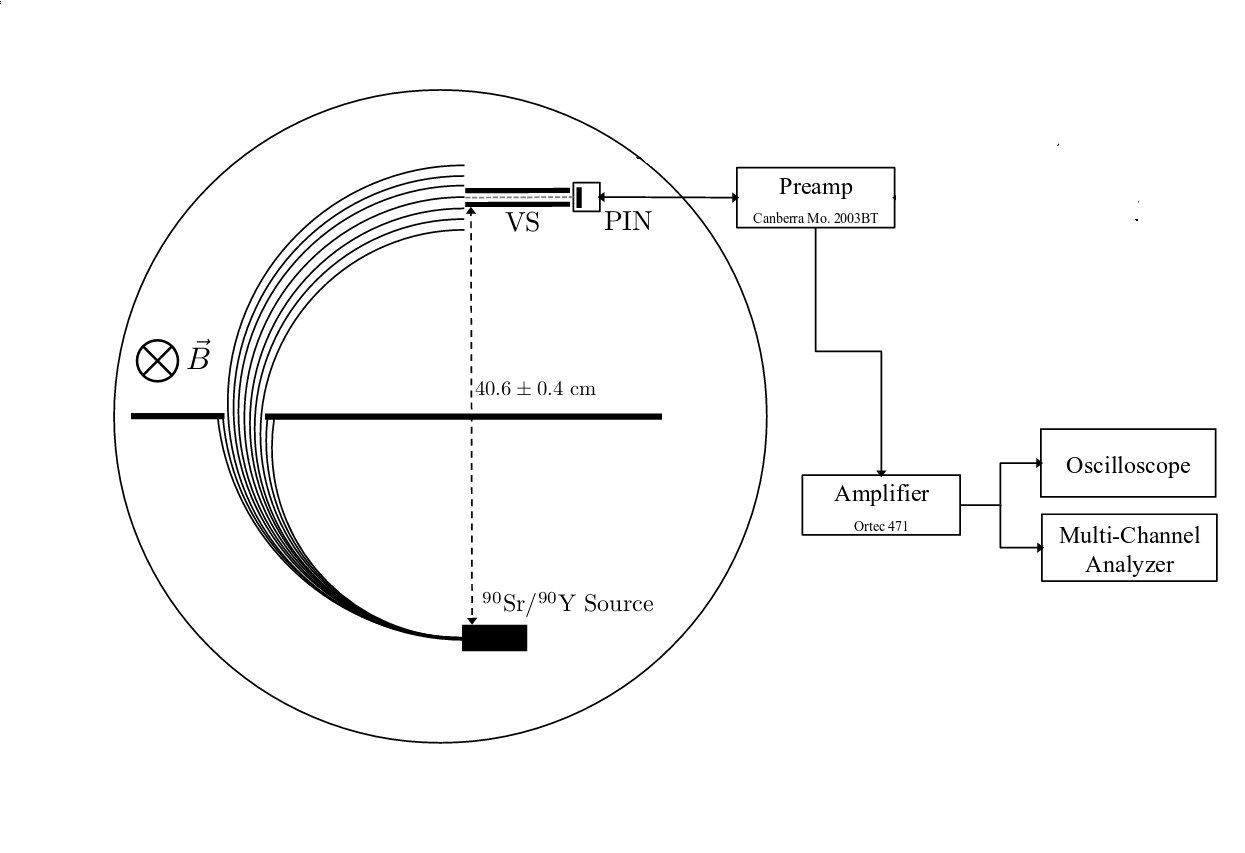
\includegraphics[width=11cm]{setup3.png}
\end{frame}

\begin{frame}
  \frametitle{Barium-133 Produces MCA Peaks at Known Energies}
  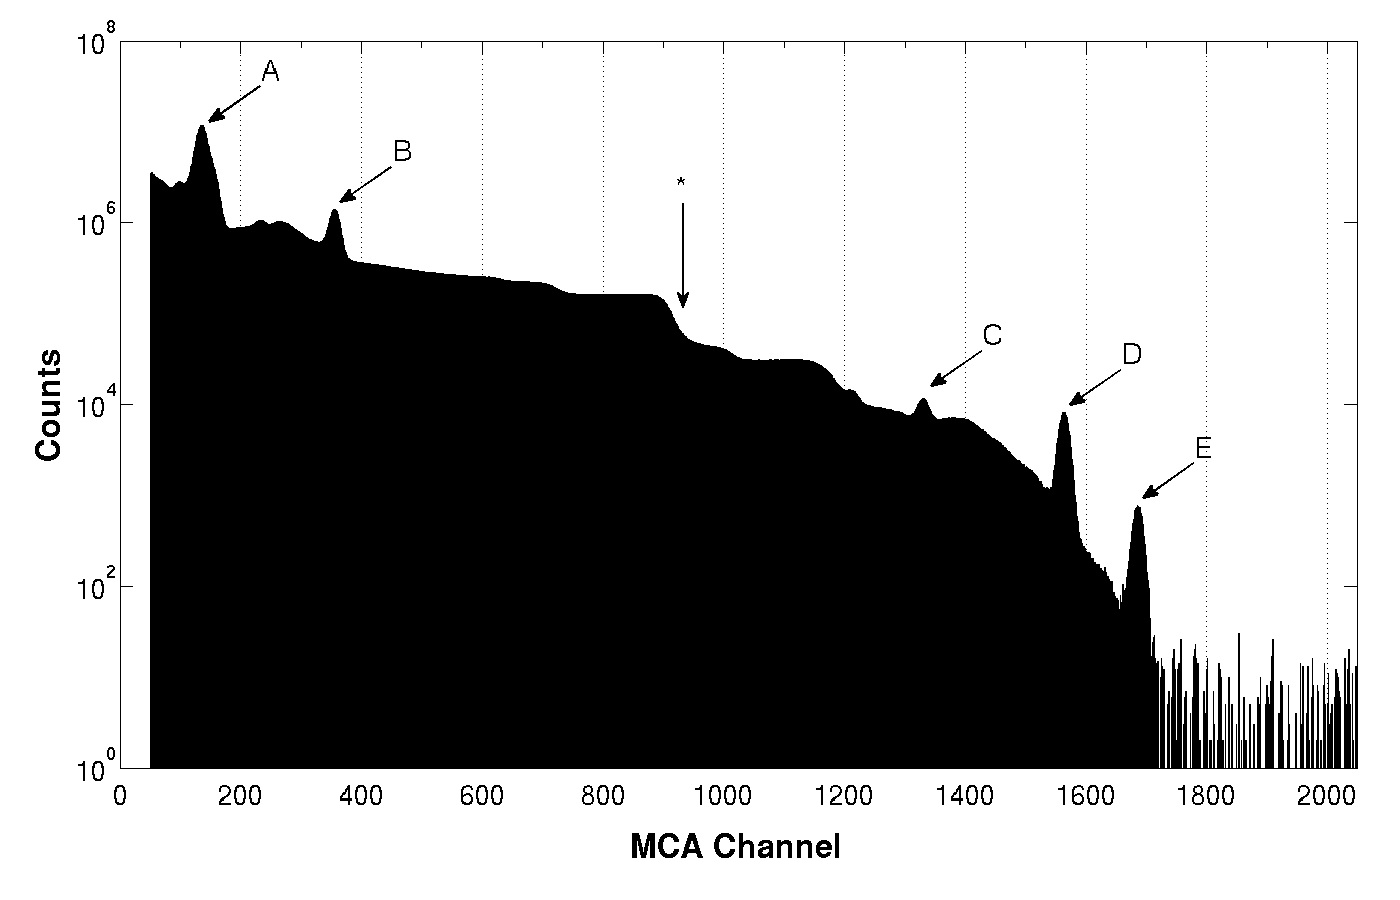
\includegraphics[width=11cm]{calibration.png}
\end{frame}

\begin{frame}
  \frametitle{MCA Readout for Sr-90/Y-90 Sharply Peaked around Energy Range}
  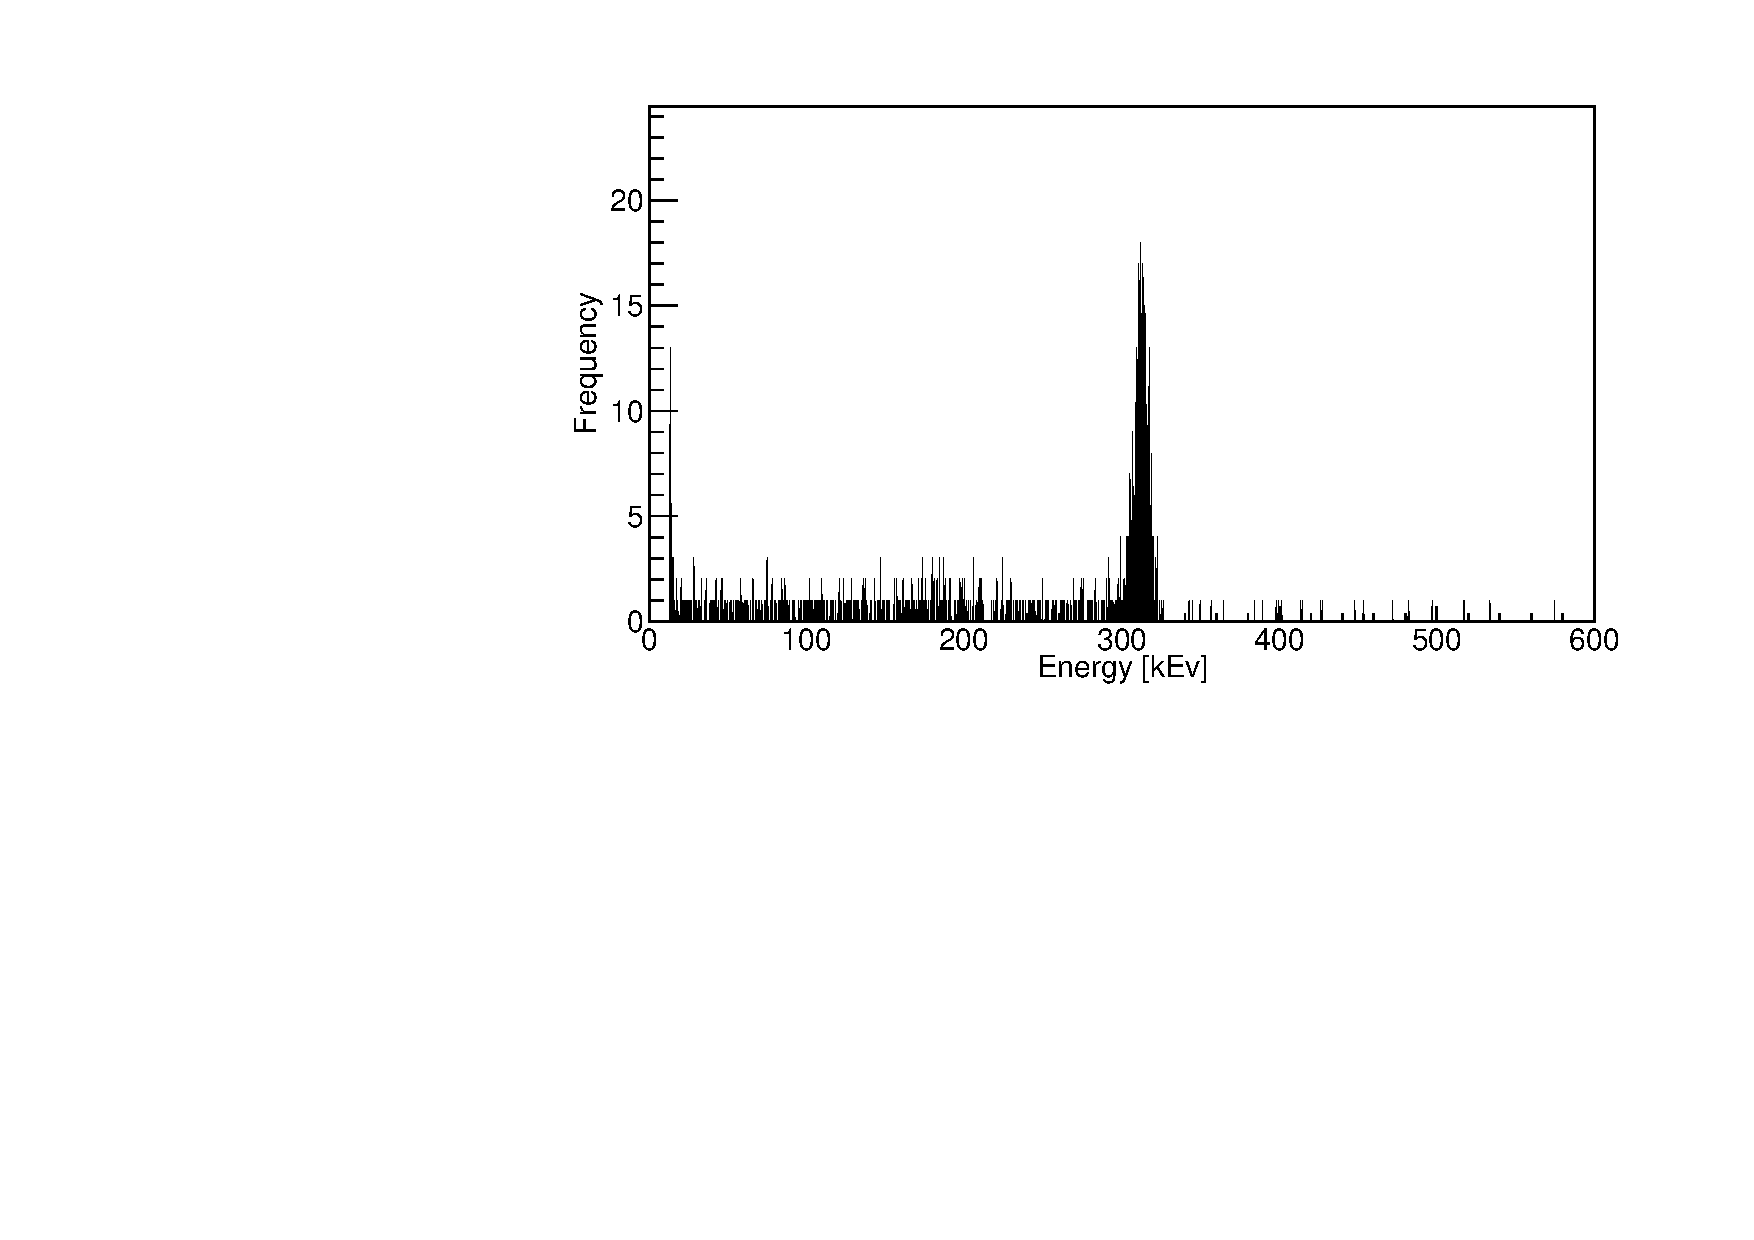
\includegraphics[width=12cm]{mca-readout-clean.pdf}
\end{frame}
\begin{frame}
  \frametitle{Magnetic Field Affects Peak Energy Range}
  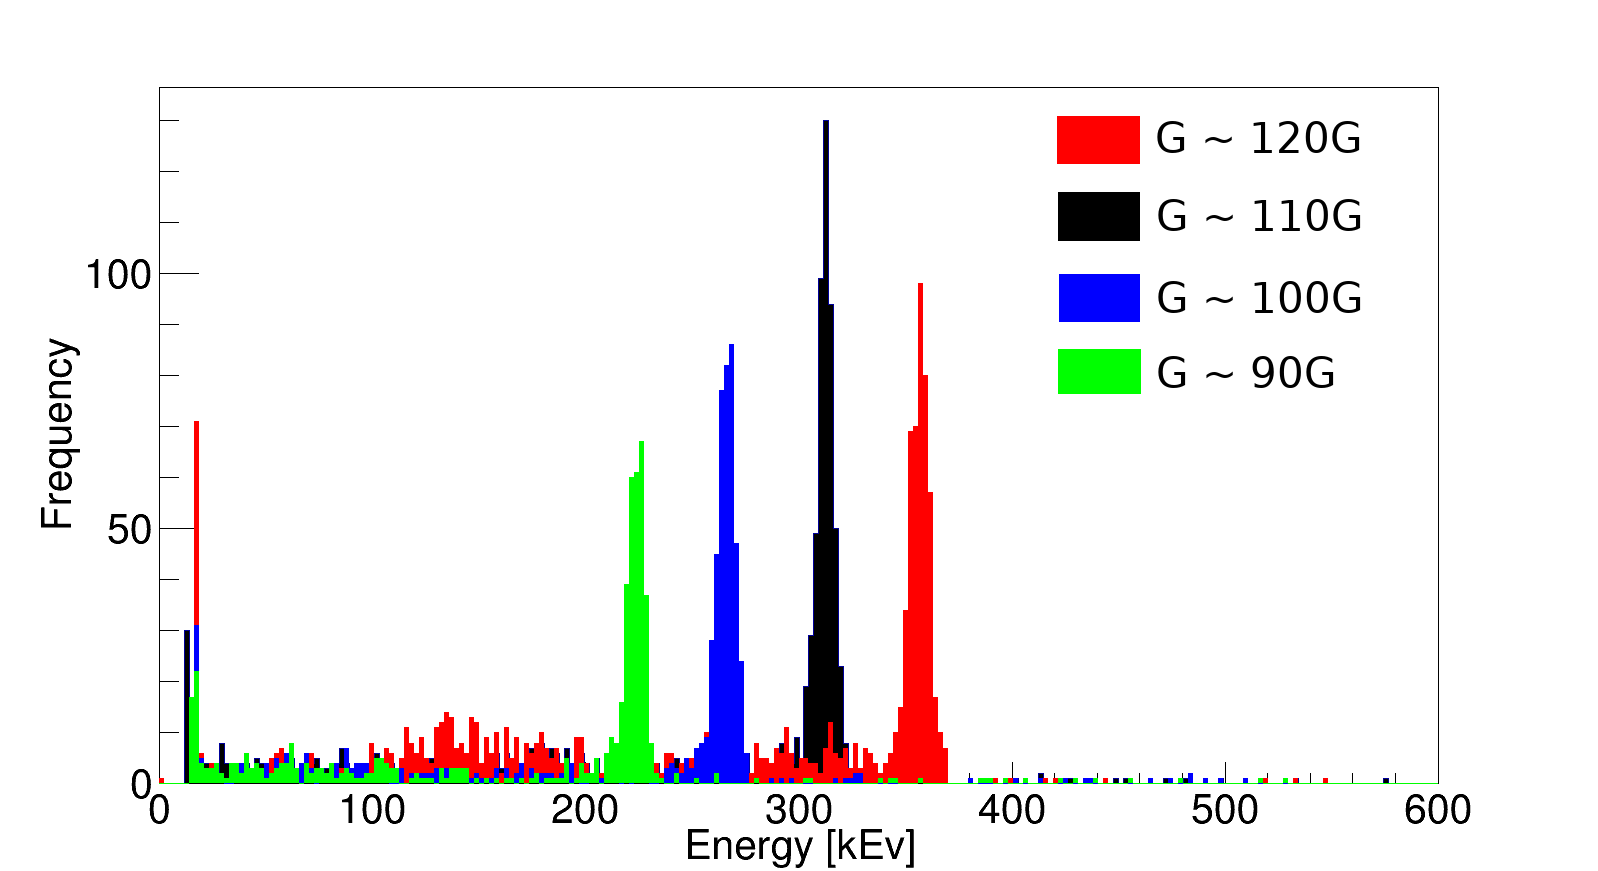
\includegraphics[width=12cm]{mca-readout-total.png}
\end{frame}

\begin{frame}
  \frametitle{Kinetic Energy Determined through Gaussian Fitting}
  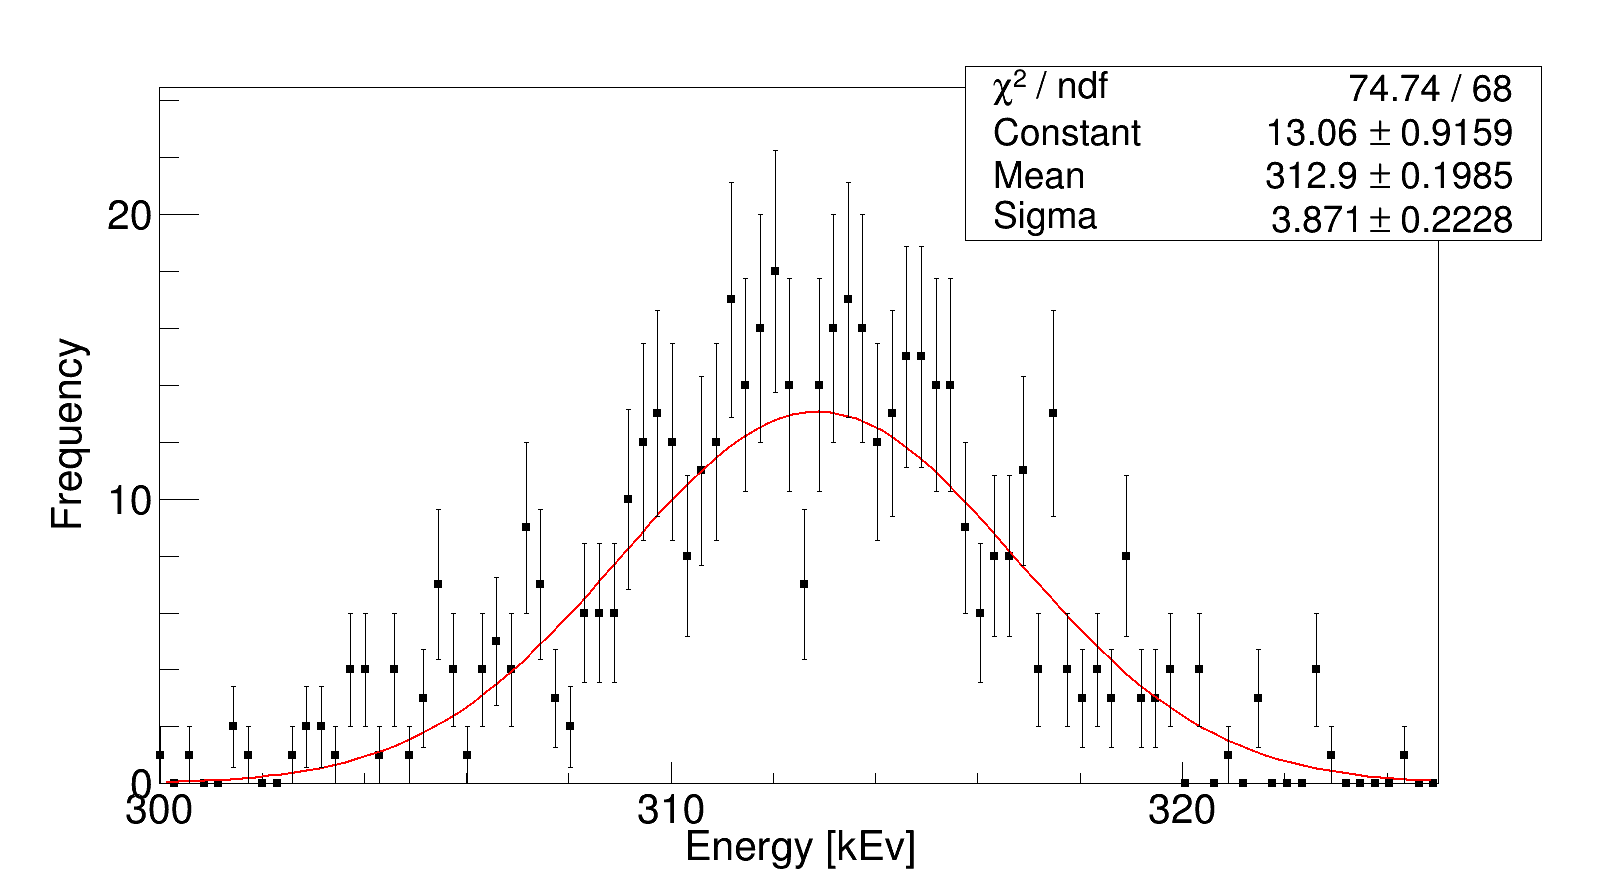
\includegraphics[width=12cm]{gaus.png}
\end{frame}

\begin{frame}
  \frametitle{Gaussian Fits Bring Uncertainty in Kinetic Energy}
  \begin{table}
  \begin{ruledtabular}
    \begin{tabular}{ccc}
      $\text{B}_{approx} \text{ (G)}$ & K (kEv) & $\sigma_K$ (kEv) \\
      \hline
      90 & 222 & .2 \\
      100 & 265 & .2 \\
      110 & 312 & .4 \\
      120 & 355 & .3 \\
    \end{tabular}
  \end{ruledtabular}
\end{table}
\end{frame}

\begin{frame}
  \frametitle{Uncertanties in Magnetic Field are Correlated}
  \textbf{Uncertainties in Magnetic Field}
\pause
  \begin{itemize}
    \item Variations during individual runs from coil heating
      \pause
    \item Variations between runs
      \pause
    \item Inhomogeneous magnetic field during individual runs
      \pause
    \item Systematic uncertainty in magnetometer
  \end{itemize}
\end{frame}

\begin{frame}
  \frametitle{Inhomogeneity Addressed by Averaging over Multiple Points}
  \begin{columns}
  \begin{column}{0.5\textwidth}
      \begin{itemize}
        \item Measured at point C during experimental runs
        \item Determined correspondance between magnetic field at point C and the average magnetic field over the path of the electron
      \end{itemize}
\end{column}
    \begin{column}{0.5\textwidth}
  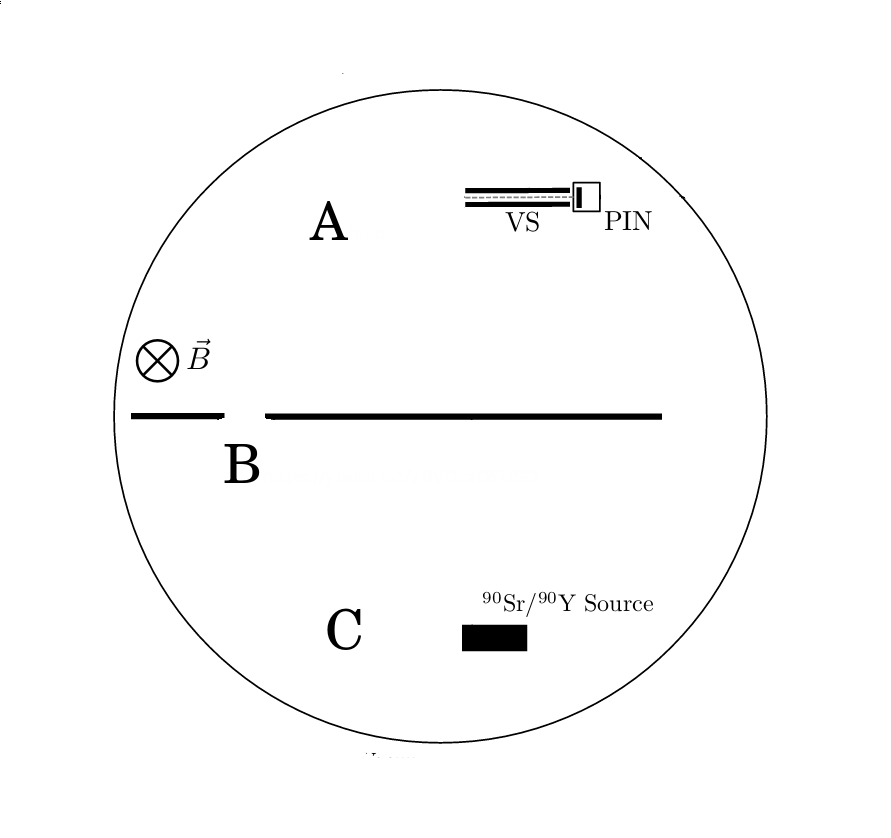
\includegraphics[width=6cm]{inhomo.png}
\end{column}
\end{columns}
\end{frame}

\begin{frame}
  \frametitle{Data Follows Relativistic Trend}
  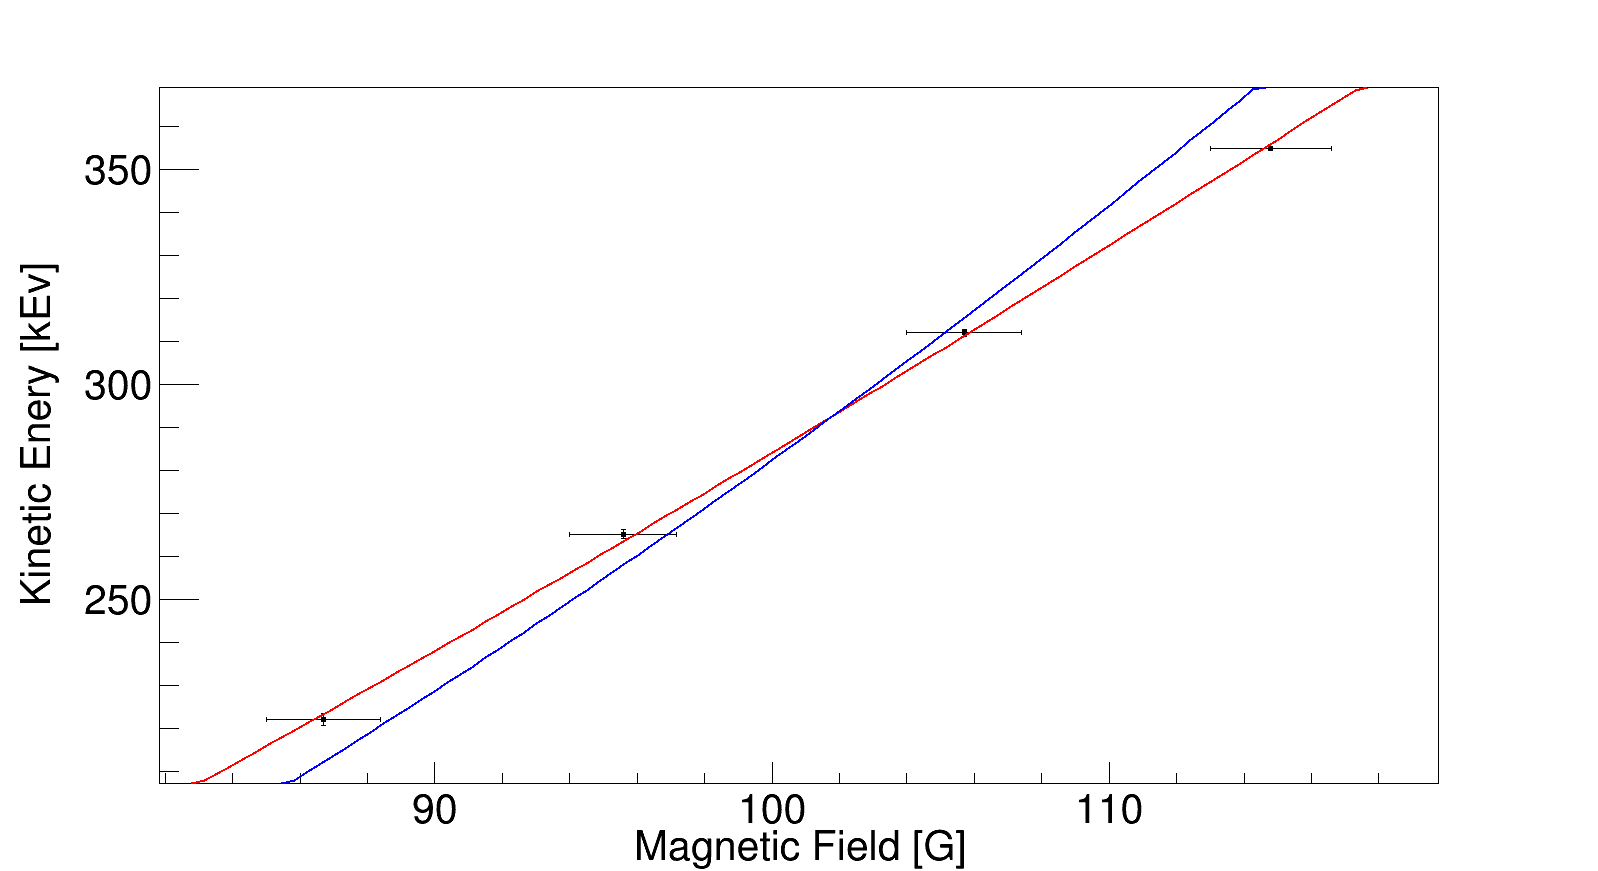
\includegraphics[width=13cm]{finalfit.png}
\end{frame}

\begin{frame}
  \frametitle{Shapes of Fit Separate at Large Kinetic Energies}
  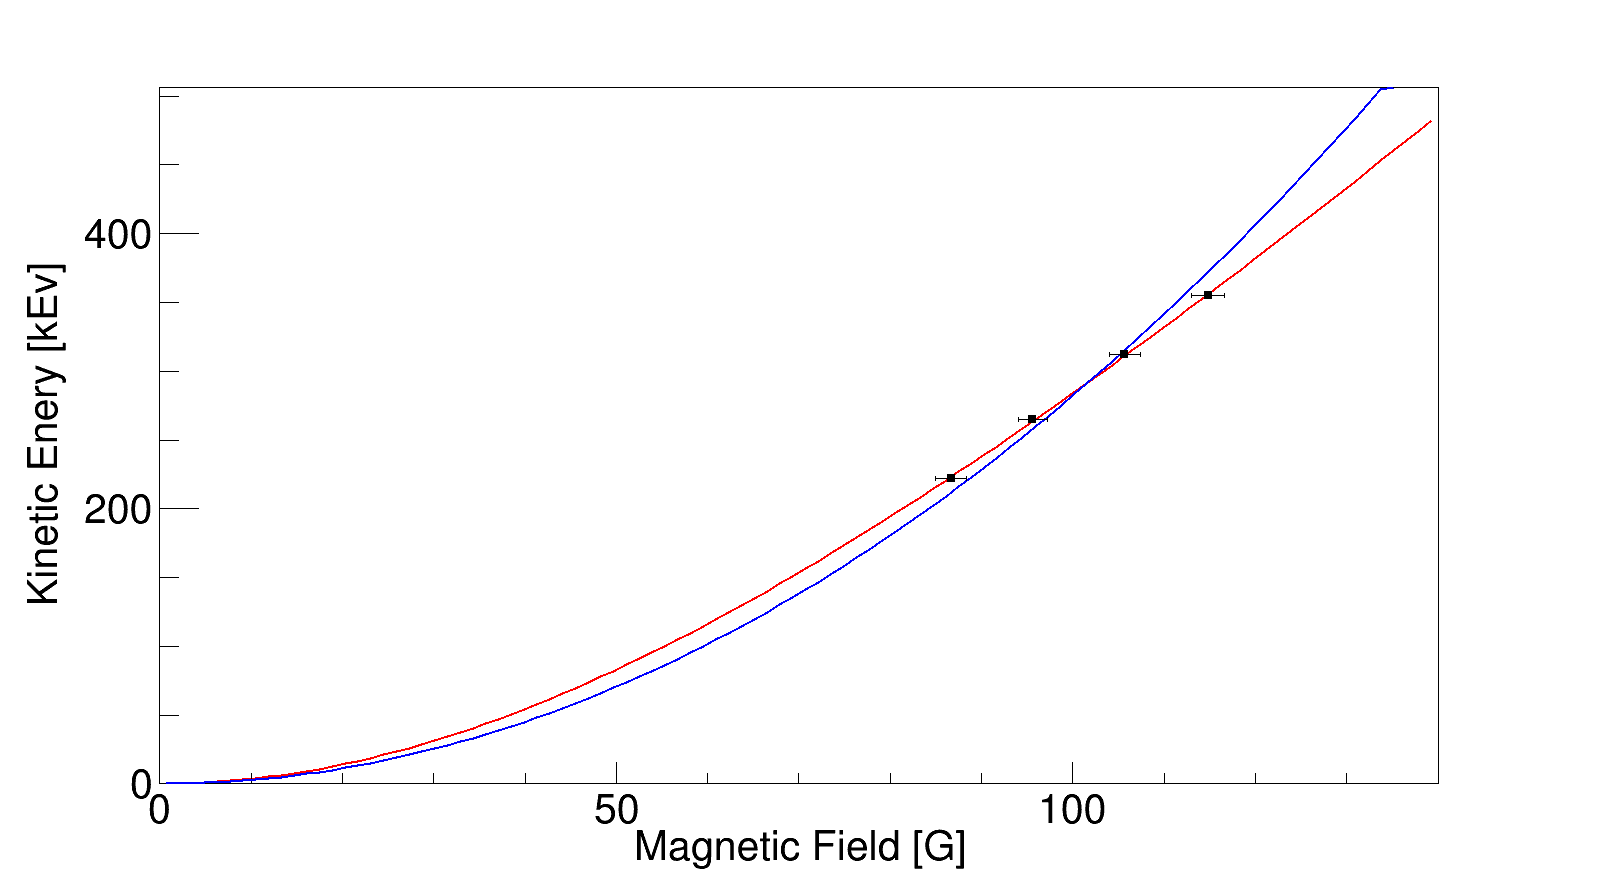
\includegraphics[width=13cm]{finalfitzoom.png}
\end{frame}

\begin{frame}
  \frametitle{Relativistic Energy Reduces to Classical when $v \ll c$}
  \begin{equation*}
    \begin{aligned}
      K &= \sqrt{p^2 c^2 + m^2 c^4} - mc^2
      \pause
      \\
      &= \sqrt{m^2c^4 \left(1 + \frac{p^2}{m^2 c^2}\right)} - mc^2
      \\
      \pause
      &= mc^2\sqrt{1 + \frac{p^2}{m^2 c^2}} - mc^2
      \\
      \pause 
      &\approx mc^2 \left(1 + \frac{p^2}{2m^2 c^2}\right) - mc^2
      \\
      \pause 
      &= \frac{p^2}{2m}
    \end{aligned}
  \end{equation*}
\end{frame}

\end{document}
